\section{Application of probabilistic catalogs for population studies}
\lb{sec:dNdS}



\begin{figure}[h]
%\hspace*{-1cm}
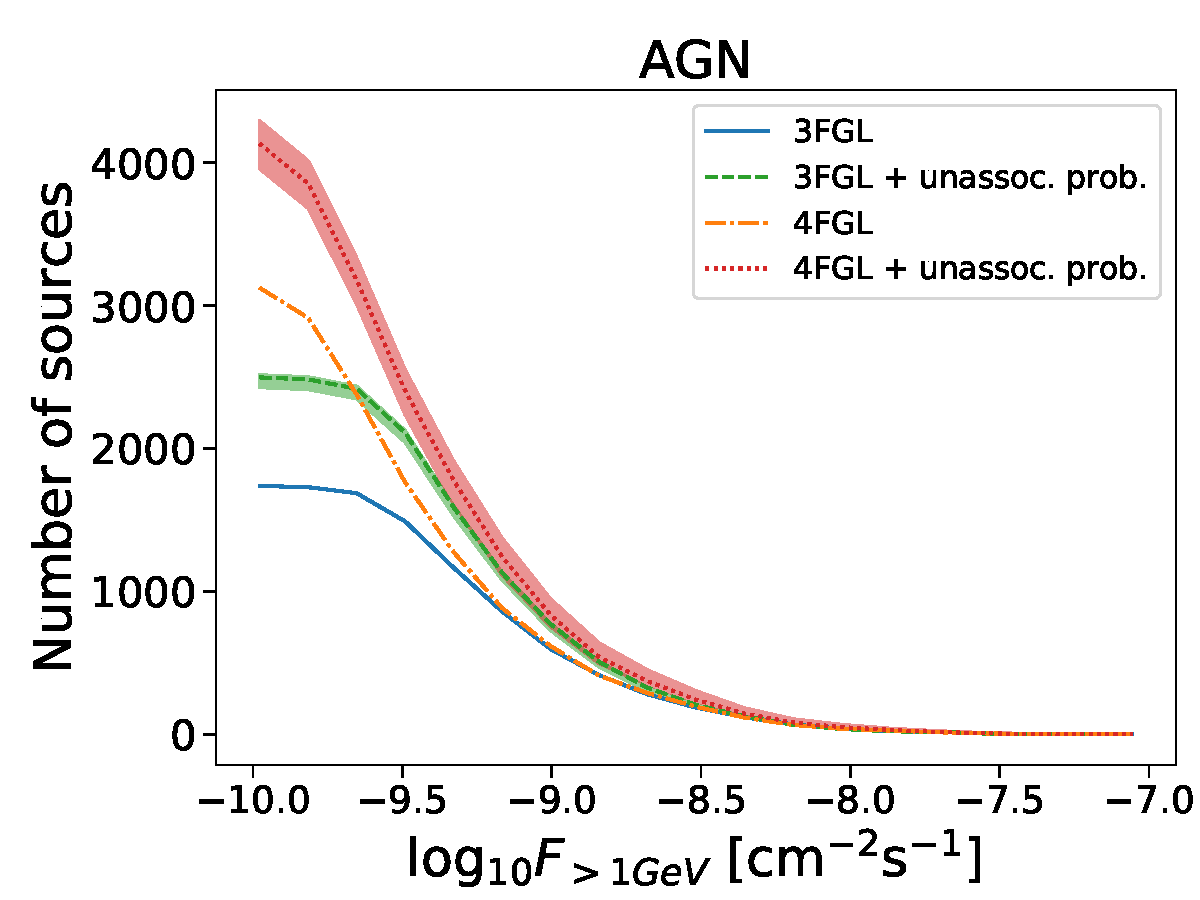
\includegraphics[width=0.4\textwidth]{plots/logN_logS_AGN.pdf}
%\hspace*{-1cm}
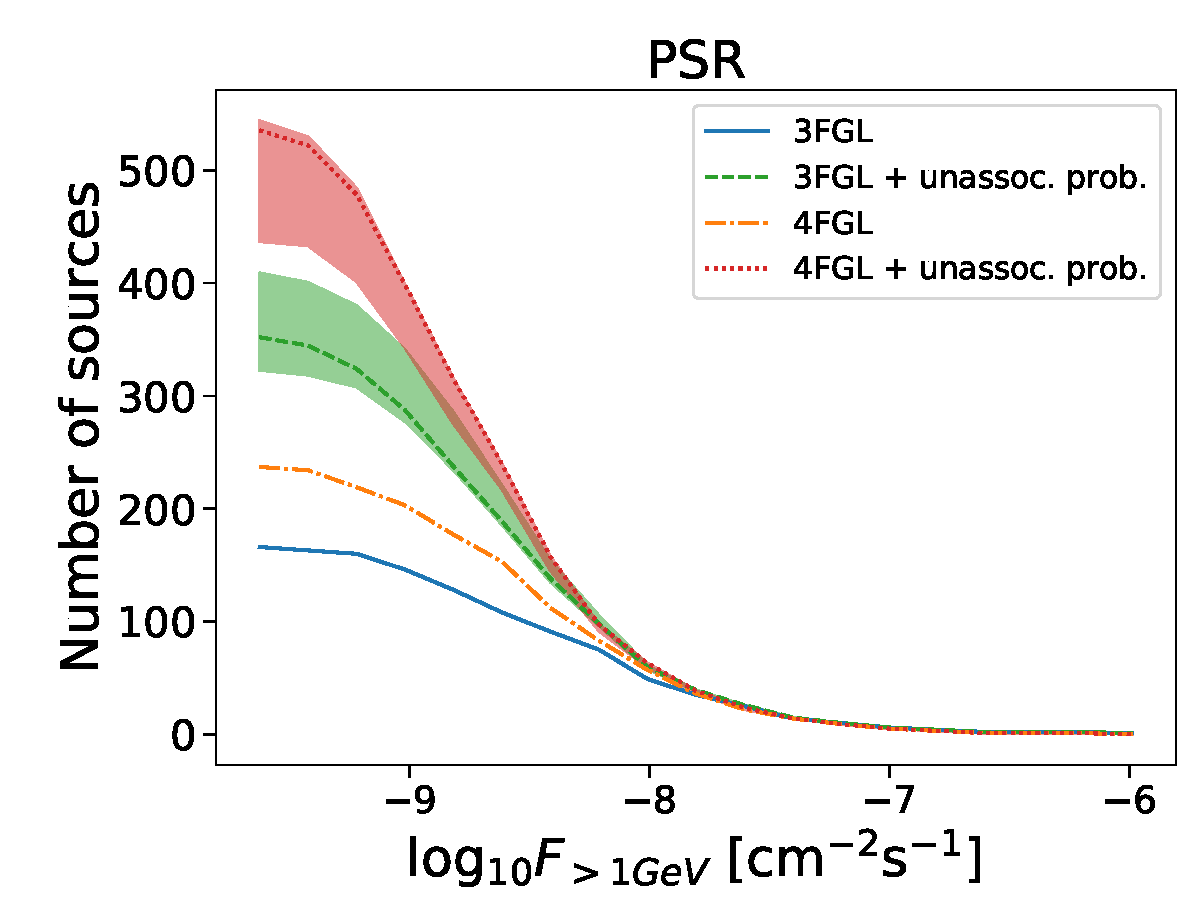
\includegraphics[width=0.4\textwidth]{plots/logN_logS_PSR.pdf}
\caption{Log N - log S.}  
\label{fig:logN_logS}
\end{figure}




\begin{figure}[h]
%\hspace*{-1cm}
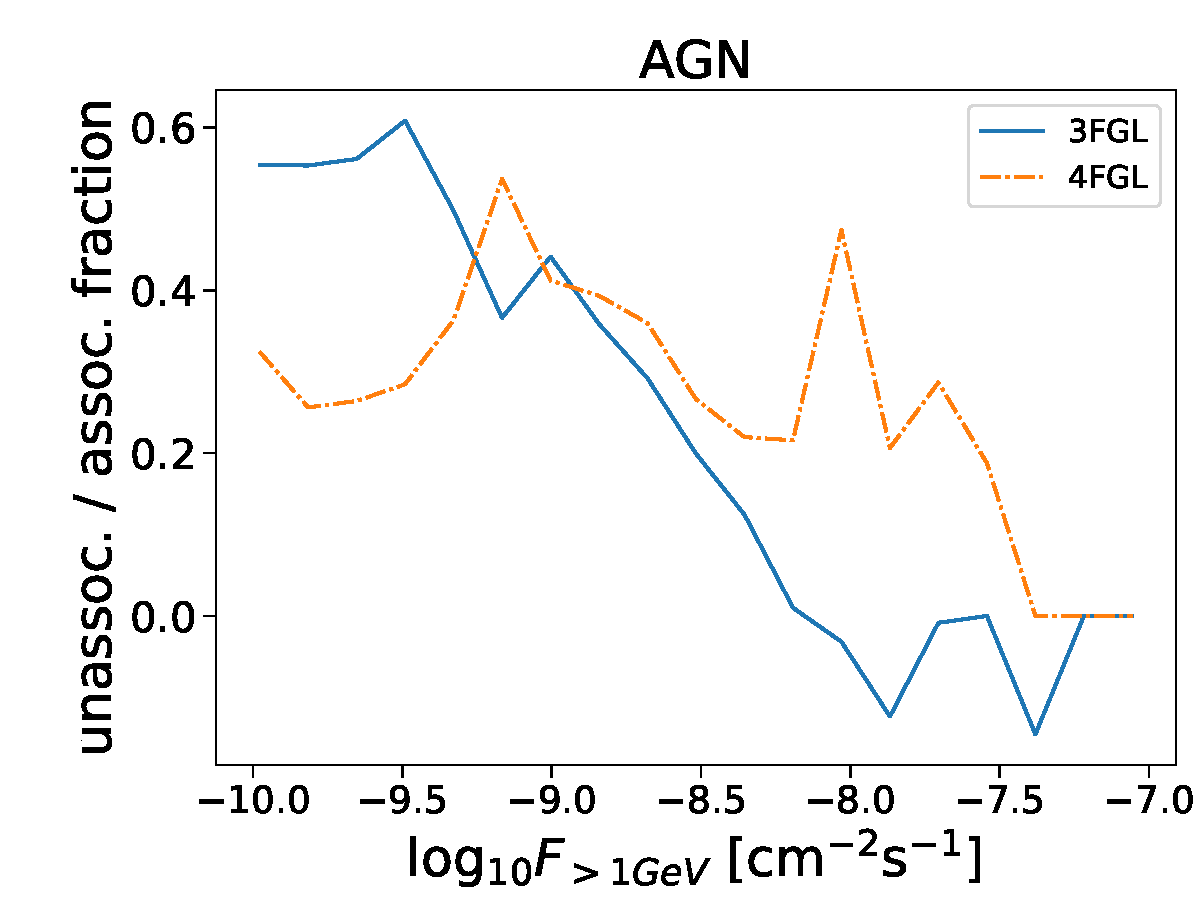
\includegraphics[width=0.4\textwidth]{plots/logN_logS_diff_AGN.pdf}
%\hspace*{-1cm}
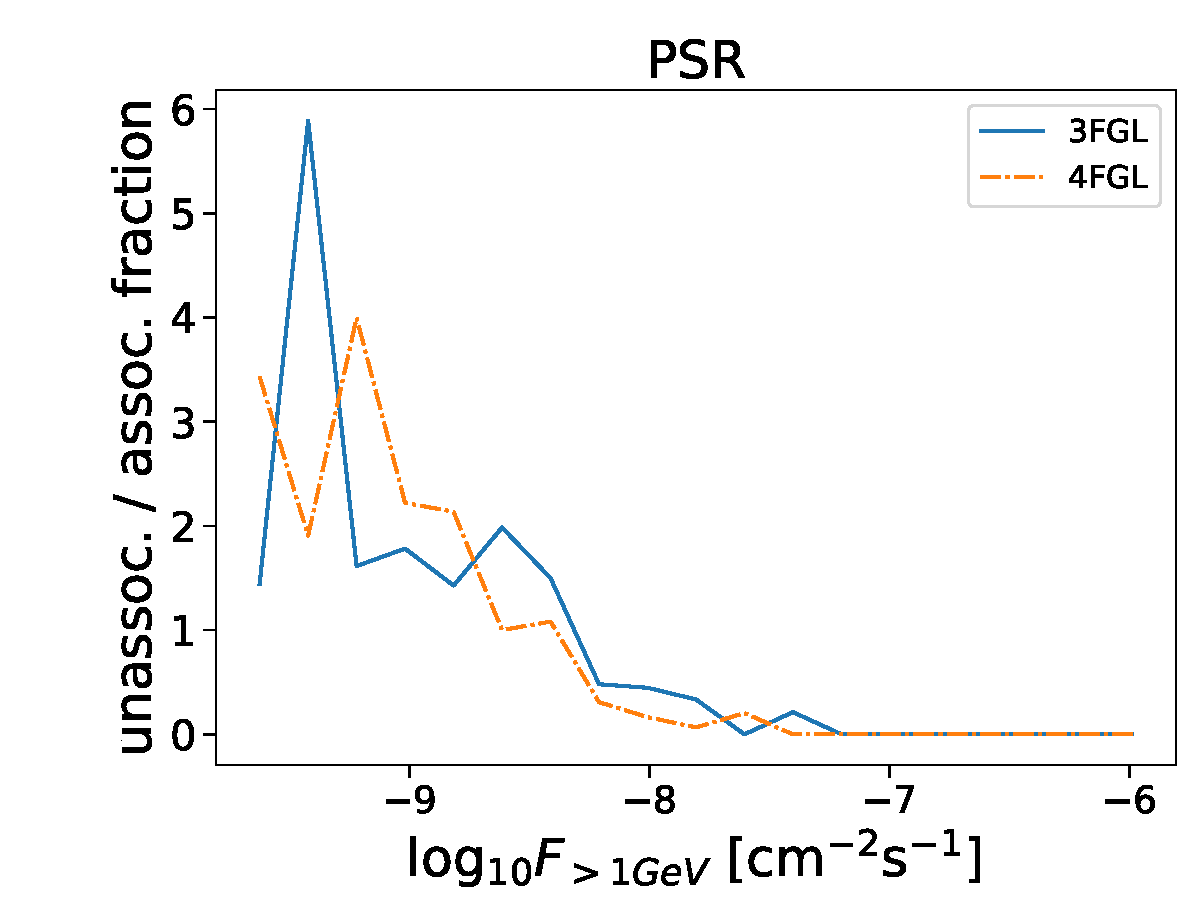
\includegraphics[width=0.4\textwidth]{plots/logN_logS_diff_PSR.pdf}
\caption{Fraction of unassociated sources relative to associated ones.}  
\label{fig:unass_vs_ass_frac}
\end{figure}



In this Section we show how probabilistic catalogs can be used, for instance, for population studies,
which can be used, for instance, to determine the contribution of unresolved point sources to isotropic gamma-ray emission.
Understanding the origin of the isotropic gamma-ray emission is important for placing strong constraints
on dark matter annihilation into gamma rays or evaporation of primordial black holes
as well as constraining the origin of astrophysical high energy neutrino flux.

